%!TEX root = ../master_thesis.tex
\chapter{Evaluation and Discussion}
\label{ch:results}
In the Chapter~\ref{ch:unvc}, we looked at the detailed formulation of our problem, network, and implementation. In this chapter, we will look at the details of the qualitative as well as quantitative evaluation of our framework. For evaluation we report the IS, FID and domain classification accuracy. For details on the IS and FID we refer to our previous discussion in Section~\ref{subsec:eval_metrics}.

Since the IS and FID require the feature space representation of the data, we developed a NN-based speaker identification network to map generated and test samples to the feature space. We then use the feature space to compute the FID which gives us a measure of the distance between the probability distribution of the test data and of the generated data. Furthermore, we use the same speaker identification network to compute the IS. In Section~\ref{subsec:sdn} we look at the details of the speaker identification network. We also evaluate the separability of the generated male and female voice samples. For this we first train a domain classifier and then use it to predict the domain of the generated samples. For a baseline, we compare the performance of the same classifier on held out test samples. In Section~\ref{subsec:dclf} we discuss the details of the domain classifier. 

In Section~\ref{sec:discussion} we discuss the results of our speech-to-speech synthesis network. We start our discussion with the first experimental setup in Section~\ref{subsec:magspecgen} where we only use the magnitude part of the time-frequency representation for training of our framework.
We have different loss terms in our network, thus to understand the effect of each term on the quality of generated samples we further perform an ablation study in Section~\ref{subsec:ablation}. In Section~\ref{subsec:full_spec_gen} we look at the results of the second setup with the full spectrogram generation. Finally, in Section~\ref{sec:discussion} we conclude the chapter with the discussion on a perceptual evaluation performed by human subjects.


%We then do the quantitative comparison of different models in Section~\ref{}. We further do the qualitative comparison of different models in Section~\ref{}. Our choice of optimization problem is composed of multiple loss function. To understand the effect of different scores we do


\section{Evaluation Setup}
\label{sec:eval_setup}
\subsection{Speaker Identification Network}
\label{subsec:sdn}
%In this section we discuss details of a speaker classifier. 
The speaker identification is defined as the task of identifying the speaker based on the segment of a speech signal. Let $K$ be the number of speakers and $N$ be the number of speech segments of $K$ speakers. For each segment $x_n$, we apply the STFT transformation and take the magnitude spectrogram $\hat{X}_n$. For every speaker $k\in K$, the spectrogram $\hat{X}\in \mathbb{R}^{F\times T}$ is a time-frequency matrix where $F$ is the number of frequency bins and $T$ is the number of time steps. Let $y$ be an indicator random variable modeling the probability of observing the $k^\text{th}$ speaker defined as:
\[
    \label{eq:indicator}
     y_{nk} = 
    \begin{cases}
   1,& \text{if the speaker label for segment $n$ is $k$}\\
    0,              & \text{otherwise}
\end{cases}
\]
Then the probability of a speaker $k$ given a spectrogram of speech segment $\hat{X}_n$ is expressed as $p(y_{nk}=1|\hat{X}_n)$. We use the multi-class cross-entropy loss and define the objective of the speaker identification task as:
\begin{equation}
    \label{eq:ll_spk}
    V = - \sum_{n=1}^N \sum_{k=1}^K y_{nk} \log (p(y_{nk}=1| \hat{X}_n))
\end{equation}

We train an end-to-end NN which takes the spectrogram representation of speech and predicts the log-likelihood probabilities of a speaker label. Our network is working at the frame level features and is based on the network proposed by \cite{okabe2018attentive}. Specifically, the spectrogram matrix $\hat{X}_n=\{\hat{X}_n^{(1)},..,\hat{X}_n^{(T)}\}$ is represented as a sequence of $T$ frames, where each frame $\hat{X}_n^{(t)}\in \mathbb{R}^F$. The network consists of three parts: 
\begin{itemize}
    \item  a time-delay neural network (TDNN) (\cite{waibel1995phoneme}) 
with three one-dimensional convolutional layers to extract frame-level features, the first layer takes input frames at $\{t-2,t-1,t,t+1,t+2\}$, the second layer takes the output of the first layer at time steps $\{t-2,t,t+2\}$ and third layer takes the output of previous layer at $\{t-3,t,t+3\}$
    \item  statistical pooling to combine frame-level features to obtain a fixed-length representation. The coefficients at frame-level features of certain frames are more relevant for discriminating speakers. To model the importance of these features we use an attention mechanism in the pooling operation. Specifically, for any segment $\hat{X}_n$, let $h_n^t$ be the hidden frames after the last TDNN layer, let $e_t$ be attention scores for each frame $h_t$ defined as a parametric transformation 
\begin{equation}
    e_t = \text{softmax} (v^T \cdot \sigma (Wh_t + b) + a)
\end{equation}
where $v\in\mathbb{R}^F$ is a weight vector, $W\in \mathbb{R}^{F\times F}$ is a weight matrix and $a$, $b$ are bias terms. The statistics $\hat{\mu}$ and $\hat{\sigma}$ of the attentive pooling is obtained as:
\begin{equation}
    \hat{\mu} = \sum_{t=0}^T e_t\cdot h_t
\end{equation}
\begin{equation}
    \hat{\sigma} = \sqrt{\sum_{t=0}^T e_t h_t \odot h_t - \hat{\mu} \odot \hat{\mu}}
\end{equation}

The fixed-length representation is obtained by concatenating $\hat{\mu}$ and $\hat{\sigma}$.
\item two fully connected dense layers of dimensionality $512$ and $256$. The output of the final dense layer is interpreted as utterance level features modeling the speech variation of a speaker.
\end{itemize}
Finally, the utterance features are passed to a softmax layer to predict the log-likelihood probabilities of speakers.
We use a LeakyReLU with a slope of $0.2$ as a non-linearity after each layer. To prevent the network from overfitting we use dropout with a probability of $0.3$ after each TDNN layer and $0.5$ after each dense layer. 

The above architecture learns utterance level features to discriminate between the speakers. Thus, by training a model on a large number of speakers we can use it to map an unseen speaker to the embedding space. For speech signals, the representations in the embedding space are interpreted as the phonetics and utterance properties of the speakers.

We use the \texttt{train-clean-100} data of the $251$ speakers from the LibriSpeech corpus. For each speaker we randomly sample a set of $70\%$ the recordings for training and the remaining $30\%$ for the evaluation of the classifier. %Figure~\ref{fig:loss_plot_dm_sp} part (b) shows the learning curve for the classifier. 
We use Adam with a learning rate of $0.001$ and momentum parameters $\beta_1=0.5$ and $\beta_2=0.999$. We use early stopping and use the classifier with the best accuracy on the $30\%$ held out samples for feature extraction. The part (b) of Figure~\ref{fig:loss_plot_dm_sp} and~\ref{fig:loss_plot_dm_sp_logmel} shows the evolution of the loss values on the training and validation set.  Table~\ref{tab:base_perform} describes the accuracy of the speaker identification network on the held out samples.

%We train the network on the LogMag and LogMel representation. We extract features after the last fully connected layer and use it to compute FID and IS. To extract features of GAN trained on Mag and Mel spectrogram  
\begin{figure}[h]
    \centering
    \subfloat[Domain Classifier]{{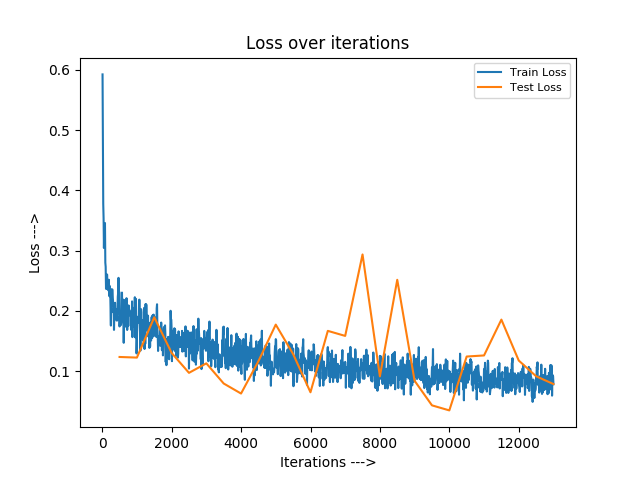
\includegraphics[width=6cm, height=5cm]{master_thesis_template/figs/loss_plot_dm_logmel.png} }}
    \qquad
    \subfloat[Speaker Identification Network]{{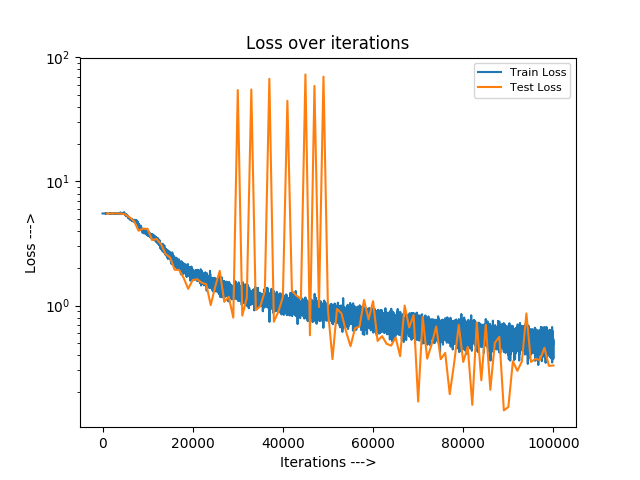
\includegraphics[width=6cm, height=5cm]{master_thesis_template/figs/loss_plot_spk_logmel.png} }}
    \caption[Loss plot of evaluation models (a)]{The loss plot of the domain classifier and speaker classifier trained on the LogMel spectrogram.}
    \label{fig:loss_plot_dm_sp_logmel}
\end{figure}

\begin{figure}[h]
    \centering
    \subfloat[Domain Classifier]{{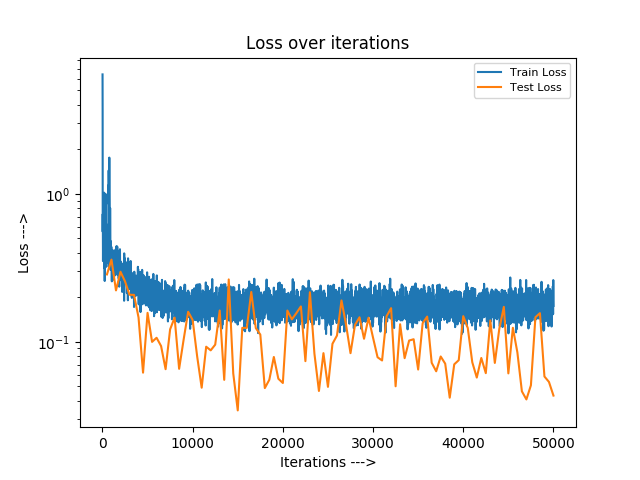
\includegraphics[width=6cm, height=5cm]{master_thesis_template/figs/loss_plot_domain_clf.png} }}
    \qquad
    \subfloat[Speaker Identification Network]{{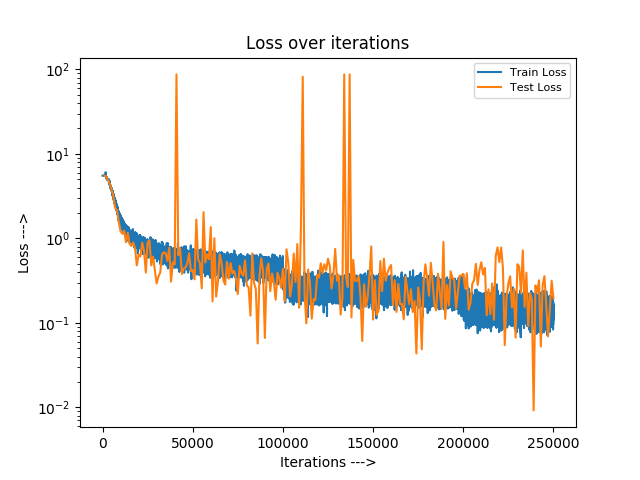
\includegraphics[width=6cm, height=5cm]{master_thesis_template/figs/loss_plot_speaker.png} }}
    \caption[Loss plot of evaluation models (b)]{The loss plot of domain classifier and speaker classifier trained on LogMag spectrogram. For better resolution we scale the loss values to $\log$ scale.}
    \label{fig:loss_plot_dm_sp}
\end{figure}

\begin{table}[]
    \centering
    \begin{tabular}{cccc}
    \toprule
\textbf{Spectrogram} & \multicolumn{2}{c}{\textbf{Test Accuracy}} \\
& Domain classification & Speaker identification \\
\midrule    
    \textbf{LogMag} & 0.975 & 0.875\\
    \textbf{LogMel} & 0.968  &0.967\\
    \bottomrule 
    \end{tabular}
    \caption[Evaluation of domain classifier and speaker identification network.]{Evaluation of the domain classifier and speaker identification network. For the domain classifier test accuracy is reported on the held out set of 40 speakers. For the speaker identification network the test accuracy is reported on 30\% held out speech samples of 251 speakers in \texttt{train-clean-100} set.}
    \label{tab:base_perform}
\end{table}

\subsection{Domain Classification}
\label{subsec:dclf}
To evaluate the quality of the generated samples we train a domain classifier network. The network is trained with an objective to discriminate between the voice of male and female speakers. We use the magnitude representation of the spectrogram for training. Let $x$ be a speech segment, $\hat{X}$ be a magnitude spectrogram, let $y_n$ be an indicator random variable defined as
\[
y_n =
\begin{cases}
    1,& \text{if $n^\text{th}$ segment is a sample of female voice} \\
    0,& \text{if $n^\text{th}$ segment is a sample of male voice} 
\end{cases}
\]
Then $p(y_n=1|X_n)$ is the probability of a sample $X_n$ belonging to the Female class. Conversely, $p(y_n=0|X_n)$ is the probability of a sample $X_n$ belonging to the male class. The learning objective for $N$ segments of speech is defined as:
\begin{equation}
    V = - \sum_{n=0}^N y_n \log(p(y_n=1|X_n)) + (1-y_n) \log(1-p(y_n=0|X_n))
\end{equation}

We implement the domain classifier as a $2$ layered perceptron network with $512$ hidden units in a first layer and $256$ units in a second layer. After each layer, we use a LeakyReLU with a slope of $0.2$ as a non-linearity. The final layer consists of a single neuron followed  by a sigmoid function to output the likelihood probability of a class. We train the network using the Adam optimizer with a learning rate of $0.0001$ and momentum parameters $\beta_1=0.5$ and $\beta_2=0.999$. In Figure~\ref{fig:loss_plot_dm_sp} and~\ref{fig:loss_plot_dm_sp_logmel} part (a) the evolution of loss values on training and validation set is shown. Table~\ref{tab:base_perform} describes the accuracy of the domain classification network on the held out set.


\subsection{Evaluation Measures}
The evaluation of the generated speech samples is a difficult task. It is not clear how to define a performance measure which correlates to the perceptual quality of speech. Therefore, we perform a quantitative as well as qualitative evaluation of the generated samples. We report all measures on the held out set of 40 speakers.

\subsubsection{Quantitative evaluation}
We report the FID and IS to evaluate the diversity of the generated samples. 
We use a speaker identification network to map translated and real samples to the feature space. We extract the features after the penultimate layer of the speaker identification network. We then use these features to compute FID and IS. To get an estimate of the range of FID and IS we also report the scores on the untrained network which serves as a measure of worst-case scenario when the network learns nothing. Table~\ref{tab:fid_is_base} describes the values of the FID and IS for an untrained network. For details on FID and IS please refer to our previous discussion in Section~\ref{subsec:eval_metrics}. 

\begin{table}[h]
    \centering
    \begin{tabular}{ccccc}
    \toprule
    \textbf{Spectrogram} &  \multicolumn{2}{c}{\textbf{FID}} & \multicolumn{2}{c}{\textbf{IS}}\\
    & \emph{min.} & \emph{untrained} & \emph{untrained} & \emph{max.} \\
    \midrule
    \textbf{LogMag} & 0 & 45140 & 1.02 & 5406\\
    \textbf{LogMel} & 0 & 25142 & 1.03 & 5406\\
    \bottomrule
    \end{tabular}
    \caption[Empirical bound on FID and IS]{Empirical bound on FID and IS. \emph{min.} stands for minimum value (is zero since FID is the distance), \emph{max.} stands for maximum value (is equal to support test size for details refer to \cite{heusel2017gans}) and \emph{untrained} is obtained from randomly initialized network.}
    \label{tab:fid_is_base}
\end{table}

We also report the domain classification accuracy which gives the measure of separability of the domain of male and female speakers. The high value of the domain accuracy means female-to-male translated samples are more like male and male-to-female translated samples are more like a female.

\subsubsection{Qualitative evaluation}
\label{sec:qualt_eval}
We use human subjects to get the evaluation of translated speech samples. We conduct two perceptual evaluation test. In the first test, we ask listeners to rate the quality of translated speech samples on a scale: Excellent (80-100), Good (60-80), Fair (40-60), Poor (20-40) and Bad (0-20). In the second test, we ask listeners to rate the extent to which each translated sample sound like a female or male person. For this we use a scale: Female (80-100), Somewhat Female (60-80), Not sure (40-60), Somewhat Male (60-80) and Male (80-100). We use webMUSHRA (\cite{schoeffler2018webmushra}) to set up the online human evaluation test.  We report the mean opinion score (MOS) for each model. The MOS is defined as an arithmetic mean of over single rating perform by human evaluators:
\begin{equation}
    \text{MOS} = \frac{\sum_{i=1}^N r_i}{N}
\end{equation}

where $r_i$ is a rating by an individual participant and N is the number of participants. We use a held out set of 40 speakers for evaluation. We translate all the samples in the held out set and randomly select a subset of 100 samples. From this subset, we arbitrarily select 11 samples of male speakers and 11 samples of female speakers. For comparison in our listening test, we present listeners with the translation of the same sample from different models. Figure~\ref{fig:perceptual_test} describe the interface of the listening test.

\begin{figure}
    \centering
    \subfloat[Quality Evaluation]{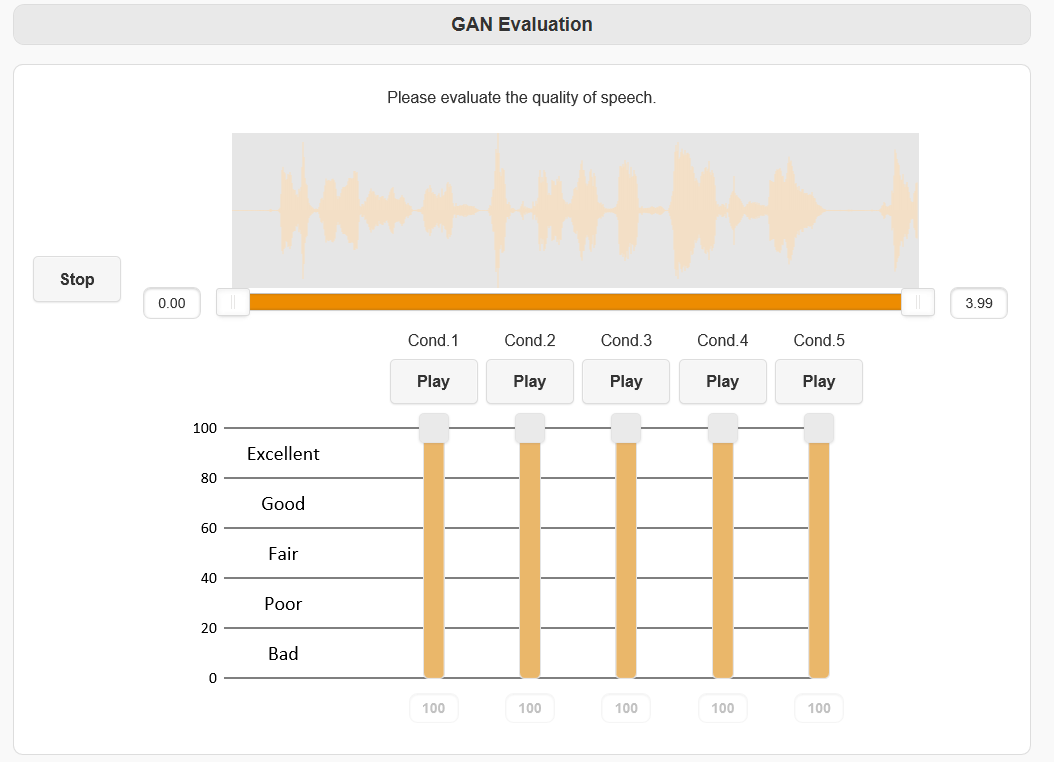
\includegraphics[width=0.45\columnwidth, height=0.45\columnwidth]{master_thesis_template/figs/mushra_ex1.PNG}}
    \hspace{10mm}
    \subfloat[Domain Evaluation]{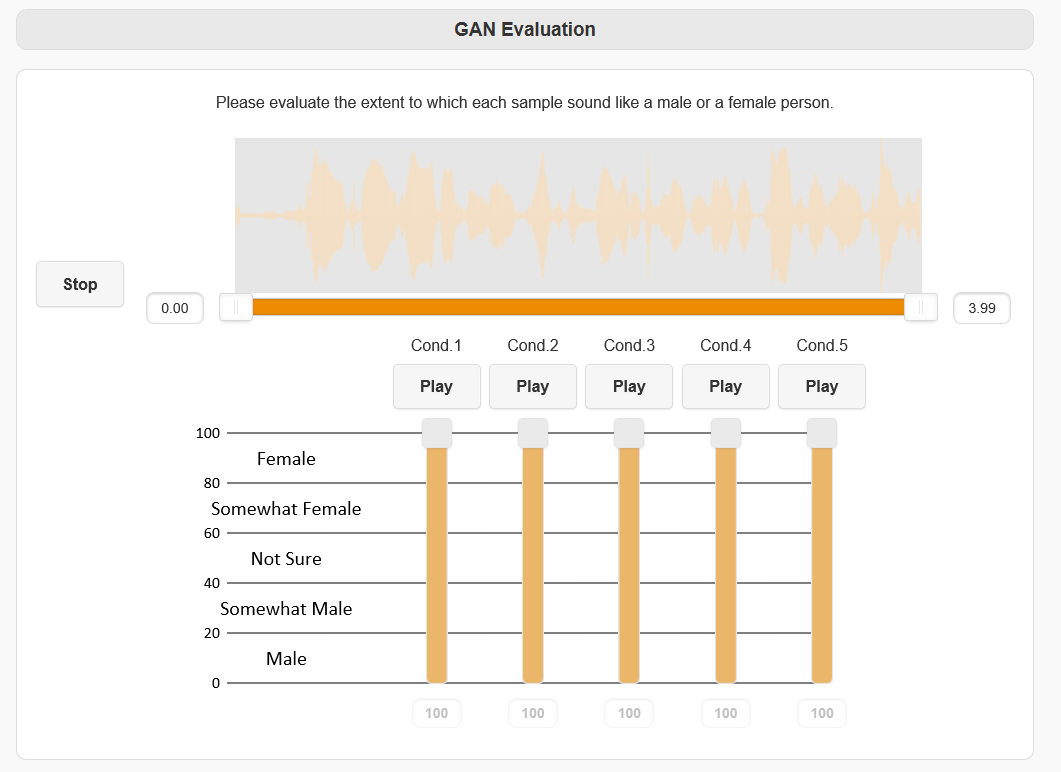
\includegraphics[width=0.45\columnwidth, height=0.45\columnwidth]{master_thesis_template/figs/mushra_ex.PNG}}
    \caption[Perceptual evaluation interface]{An example of the GUI we used for the perceptual evaluation. In the domain evaluation for male speakers we subtract reported scores from 100. This way we end up with the same scale for male and female speakers.}
    \label{fig:perceptual_test}
\end{figure}{}

\subsection{Robustness of FID and IS}
\label{subsec:robust_scores}
To further interpret the FID and IS scores we perform the robustness analysis. We add increasing disturbance to generated samples and see the effect on FID and IS. We apply the following disturbance on the spectrogram:

\begin{itemize}
    \item \textbf{Gaussian noise}: For a spectrogram $\hat{X}$, we compute a noisy version $(1-\alpha) \hat{X} + \alpha \eta$, where $\eta\sim \mathcal{N}(0,1)$ is sampled from Gaussian noise with zero mean and unit variance where $\alpha$ is a parameter to control the mix of signal and noise. This noise has a degrading effect on the quality of the speech signal. A higher fraction of noise results in low signal to noise ratio.

    \item \textbf{Salt and pepper noise}: For a spectrogram $\hat{X}$ we randomly flip the coefficient values with a probability $\alpha$. We set the coefficient value to $0$ or $1$ with a probability of $0.5$. This results in peaks in the spectrogram representation. These peaks affect the perceptual quality of sound giving the robotic nature to the sound. 
\end{itemize}

    \begin{table}[h]
    \centering
    \begin{tabular}{ccc}
    \toprule
    $\alpha$ (Noise parameter) & \textbf{FID} & \textbf{IS}\\
    \midrule
    0     &  28.57& 19.86\\
    0.1     & 192.49& 23.73\\
    0.25&  602.18 & 81.16\\
    0.50 & 1715.17& 1898.26\\
    0.75 & 3567.12& 1823.59\\
    \bottomrule 
    \end{tabular}
    \caption[Robustness of the FID and IS score to Gaussian Noise]{FID and IS score with increasing Gaussian noise for the VC-Con-GAN. Here we consider a joint distribution of male and female speakers.}
    \label{tab:qualt_gn}
\end{table}

\begin{table}[h]
    \centering
    \begin{tabular}{ccc}
    \toprule
    $\alpha$ (Noise parameter) & \textbf{FID} & \textbf{IS}\\
    \midrule
       0  &  28.57& 19.86\\
       0.1 & 1466.67 & 631.03\\
       0.25 &5029.97 & 1.18\\
       0.50 &11691.86 & 1.04\\
       0.75 &16804.00 & 1.03\\
     \bottomrule  
    \end{tabular}
    \caption[Robustness of the FID and IS score to salt and pepper noise]{FID and IS score with increasing salt and pepper noise for the VC-Con-GAN. Here we consider a joint distribution of male and female speakers.}
    \label{tab:qualt_sp}
   \end{table}


Table~\ref{tab:qualt_gn} and~\ref{tab:qualt_sp} describe the FID and IS score for different values of the noise factor $\alpha$. We can see the FID score is consistent with the increasing noise. On the other hand, the IS has a strange behavior since it increases for Gaussian noise and fluctuates for salt and pepper noise. %The effect on IS is is contrary to the expectation. 
The robustness of the FID score for Gaussian noise implies the metric is correlated to signal to noise ratio and the salt and pepper noise indicates that the FID is also robust to capture a difference between natural and robotic sounding voice. For the above reason, we will build our discussion on the FID. For the sake of completeness, we also report the IS but we do not use it for further discussions.


\section{Results and Discussion}
\label{sec:discussion}
In this section, we look at the results and compare the performance of the different models. We refer to the base UNIT network as VC-GAN, the network with the consistency loss discussed in Section~\ref{subsec:spec_con} as VC-Con-GAN, and the network with the projection-based consistency loss discussed in Section~\ref{subsec:gl_spec_con} as VC-GL-GAN. 

\subsection{Magnitude spectrogram generation}
\label{subsec:magspecgen}
In this section, we focus our discussion on the first setup where we only use the magnitude part of the STFT representation.
Table~\ref{tab:eval_gan_mag} compares the performance of the VC-GAN and VC-Con-GAN for different magnitude scales. For the VC-Con-GAN we train the network only on the magnitude and log-magnitude scale and omit on the mel scale. This is because the consistency constraint of the spectrogram only holds on these two representations.

We separately report the FID scores for female and male domain. We observed the log transformation generally helps the training and provides lower FID scores. In the spectrogram representation, the low-frequency components are associated with the information and the high-frequency components are associated with noise. The log transformation spread the spectrogram by enhancing the lower components and compressing the noise part. We attribute the better performance of the log scale to the enhancement of speech information which makes it easier for NNs to learn meaningful features. 

The VC-Con-GAN outperforms the VC-GAN in terms of FID scores. The best value of the FID is achieved for the log magnitude representation. The introduction of the consistency loss provides an improvement over the base model.

In Figure~\ref{fig:spec_translate} we show an example of a spectrogram of a four second segment of the original speaker and the corresponding translated version. We show the plot of our best model VC-Con-GAN trained on the log magnitude spectrogram. We can see the network learn to shift the tones as well as learn to change the shape and spacing of contours to translate the voice. 
\begin{table}[h]
    \centering
    \begin{tabular}{cccccc}
    \toprule
    \textbf{Method}     & \textbf{Spectrogram} & \textbf{IS} & \multicolumn{2}{c}{\textbf{FID}} & \textbf{Accuracy}\\
    & & & Female & Male & \\
    \midrule
     \textbf{VC-GAN}    & Mag & 22.14 &130.32 & 100.36 & 0.894 \\
         & Mel & 30.64& 123.79&89.16 & 0.935\\
         & LogMag &21.35 &$\textbf{76.90}$ &$\mathbf{74.18}$& 0.935\\
         & LogMel &32.06& 127.14&116.13& $\mathbf{0.938}$\\
    \midrule
     \textbf{VC-Con-GAN}    & Mag & 22.89 &94.83 & 83.52 &  $\mathbf{0.928}$\\
%         & Mel & & &\\
         & LogMag & 19.86 & $\mathbf{70.11}$& $\mathbf{69.50}$ & 0.860\\
    \bottomrule 
    \end{tabular}
    \caption[Evaluation of generated samples of different GANs trained on Magnitude spectrogram.]{Evaluation of generated samples of different GANs trained on Magnitude spectrogram. We compare IS, FID and domain classification accuracy. We use held out set of 40 speakers for evaluation.}
    \label{tab:eval_gan_mag}
\end{table}

\begin{figure}[h]
    \centering
    \subfloat[Spectrogram: Female to Male]{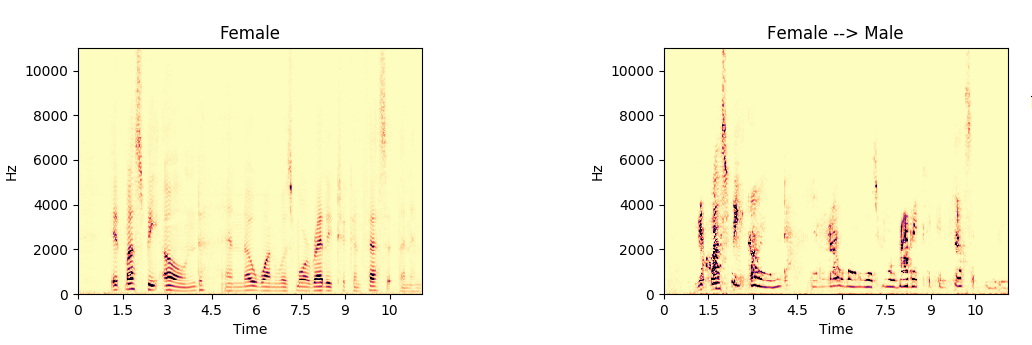
\includegraphics[width=0.95\columnwidth, height=0.35\columnwidth]{master_thesis_template/figs/f2m.png}}
    \\
    \subfloat[Spectrogram: Male to Female]{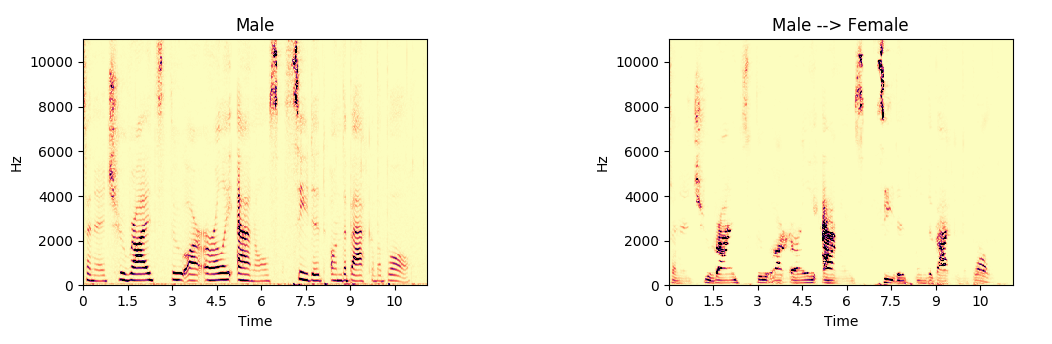
\includegraphics[width=0.95\columnwidth, height=0.35\columnwidth]{master_thesis_template/figs/m2f.png}}
    \caption[Examples of spectrogram translations.]{An example of spectrogram translation from female to male at the top and male to female at the bottom.}
    \label{fig:spec_translate}
\end{figure}{}


% VC-GAN but attains a lower domain accuracy. The lower domain accuracy can be explained by high diversity in generated samples
 




\subsubsection{Ablation Study}
\label{subsec:ablation}
We have several loss functions in our optimization problem. To understand the direct effect of each term on the quality of the generated samples, we perform an ablation study. In this study, we remove the respective loss term and observe the effect on the FID and domain classification accuracy. Table~\ref{tab:ablation_study_acc} describes the effect on FID scores and Table~\ref{tab:ablation_study_fid} describes the effect of loss terms on domain accuracy. The removal of the spectrogram consistency loss results in an increase of FID scores for the magnitude as well as the log magnitude scale. We observed that the effect on the domain accuracy is not consistent. It decreases for the magnitude and increases for the log magnitude. The explanation for this is not clear. We think this also depends on the generalization of the base domain classifier. Henceforth, for the evaluation of the generated samples, we do not rely on the classification accuracy. We use it as a sanity measure to check whether voice samples are translated across the domain. We will later see in Section~\ref{subsec:human_eval} the FID scores are also consistent with the human evaluation. Thus, we conclude that the FID is a better measure for the evaluation. 

The other loss terms follow from the base UNIT network and have a varying effect for different input representations. The KL loss term in the VAE does not provide any improvement in terms of the FID. The cycle consistency term is useful for the magnitude representation but not for the mel, log magnitude, and log mel representation. We claim this is due to the weight sharing condition which also ensures a pair of corresponding samples in the two domains are represented by the same latent features. To support our claim we removed the cycle consistency loss, as well as the weight sharing. In this case, we observed that all networks fail at the task of domain translation. 

\begin{table}[h]
    \centering
    \begin{tabular}{cccccc}
    \toprule
    \textbf{Spectrogram} &\textbf{Full Loss} & \textbf{No Con} & \textbf{No VAE} & \textbf{No CC} &\textbf{No Shared-CC}\\
    \midrule
    \textbf{Mag} &0.928& 0.894 & 0.889&0.500 & 0.499 \\
    \textbf{Mel} &- &0.935 & 0.906& 0.953 & 0.000\\
    \textbf{LogMag} &0.860 & 0.935 &0.928 & 0.726& 0.499\\
    \textbf{LogMel} & - &0.938&0.939&0.909 & 0.500 \\
    \bottomrule 
    \end{tabular}
    \caption[Ablation study: Domain accuracy]{Effect of different loss terms on the domain accuracy where full loss represent our VC-Con-GAN model, NoCon is obtained by removing the spectrogram consistency loss, No VAE is obtained by removing the VAE loss, No CC is obtained by removing the cycle consistency loss term and No shared-CC is obtained by removing the weight sharing condition and the cycle consistency loss.}
    \label{tab:ablation_study_acc}
\end{table}
\begin{landscape}
\begin{table}
    \centering
    \begin{tabular}{ccccccccccc}
    \toprule
    \textbf{Spectrogram} &\multicolumn{2}{c}{\textbf{Full Loss}} & \multicolumn{2}{c}{\textbf{No Con}} & \multicolumn{2}{c}{\textbf{No VAE}} & \multicolumn{2}{c}{\textbf{No CC}} &\multicolumn{2}{c}{\textbf{No Shared-CC}}\\
    & Female & Male & Female & Male & Female & Male & Female & Male & Female & Male\\
    \midrule
    \textbf{Mag} &94.83& 83.52& 130.32& 100.36 & 87.08 & 81.57 & 2491.03&1273.12& 408.45&4209.07\\
    \textbf{Mel} &- &- & 123.79& 89.28 &139.22 & 91.99 &103.83&112.37&1546.00&779.61\\
    \textbf{LogMag} &70.11 & 69.50 & 76.90  & 74.18 & 74.88& 69.14 & 94.71& 108.09 & 420.11 & 730.16\\
    \textbf{LogMel} & - & - & 127.14 & 116.01 & 94.31 & 98.51&122.67&97.74 &2310.52& 461.62\\
    \bottomrule 
    \end{tabular}
    \caption[Ablation study: FID]{Effect of different loss terms on FID scores where full loss represents our VC-Con-GAN model, NoCon is obtained by removing the spectrogram consistency loss, No VAE is obtained by removing the VAE loss, No CC is obtained by removing the cycle consistency loss term and No CC-VAE is obtained by removing the weight sharing, VAE as well as the cycle consistency loss term. }
    \label{tab:ablation_study_fid}
\end{table}
\end{landscape}


\subsection{Full spectrogram generation}
\label{subsec:full_spec_gen}
The quantitative evaluation of this setup is difficult. It is mainly due to the difficulties associated with obtaining the feature space representation of the full spectrogram. The speaker identification network discussed in Section~\ref{subsec:sdn} fails to learn from the full spectrogram. We think an additional phase part serves as noise and introduces additional difficulties in the learning task since the speaker identification task relies on features which are dependent on phonetic variations or the accent of a speaker and these features can be independently obtained from the magnitude spectrogram. Thus for quantitative evaluation, we discard the phase part and only use the magnitude part to get the feature representation to compute the FID and IS. Likewise, we only use the magnitude part to report the domain classfication accuracy. Since we only use the magnitude spectrogram for the evaluation we don't rely on these results and only report them for the sake of completeness. For this part we mainly focus on the perceptual evaluation discussed in following section. Table~\ref{tab:eval_gan_full} describes the performance of this setup.  

%We observed the log scaling also performs better in this setup. The consistency loss provides an improvement in FID for female speaker but not for male speaker. We think this could be improved by tuning hyperparameter of consistency loss which we leave as future work.

\begin{table}[h]
    \centering
    \begin{tabular}{cccccc}
    \toprule
    \textbf{Method}     & \textbf{Spectrogram} & \textbf{IS} & \multicolumn{2}{c}{\textbf{FID}} & \textbf{Accuracy}\\
    & & & Female & Male & \\
    \midrule
     \textbf{VC-GAN}    & MagIF &19.73 & 81.13& 65.34 & 0.819 \\
         & LogMagIF& 15.33&$\mathbf{70.58}$ &$\mathbf{57.01}$ &0.783\\ 
    \midrule
     \textbf{VC-Con-GAN}    & MagIF &19.46 &74.14 &78.03 &0.868 \\
         & LogMagIF & 17.66& $\mathbf{59.38}$&$\mathbf{75.40}$ & 0.843\\
    \midrule
     \textbf{VC-GL-GAN}  & MagIF &19.56 &71.57& 77.76& 0.933\\
         & LogMagIF &18.60&$\mathbf{62.25}$ &$\mathbf{73.26}$ & 0.880\\          
    \bottomrule 
    \end{tabular}
    \caption[Evaluation of generated samples of different GANs trained on the full-spectrogram.]{Evaluation of generated samples of different GANs trained on the full-spectrogram. We compare the Inception Score (IS), Fr\'{e}chet Distance (FID) and domain detection accuracy. We report the accuracy on unseen original test samples and generated samples.}
    \label{tab:eval_gan_full}
\end{table}




\subsection{Human Evaluation}
\label{subsec:human_eval}
For the qualitative evaluation of each model, we select the spectrogram with the best FID scores. We do the perceptual evaluation of these models using the scales discussed in Section~\ref{sec:qualt_eval}. There were $28$ participants in the study.
Table~\ref{tab:mos} compares the MOS of the different models. Figure~\ref{fig:mos_quality_domain} compares the histogram of the different models with $95\%$ confidence interval.

The consistency loss with the log magnitude representation performs best in terms of the quality as well as the domain translation. Furthermore, the results are also consistent with the FID scores. For the second setup, we observed the results are not good in terms of the quality and much worse than the magnitude-based representations. But in terms of the domain translation the results are comparable. The two different consistency terms used in this case provide an improvement over the base model. The consistency of the magnitude spectrogram performs better than the projection-based consistency condition of the full spectrogram. The explanation is not clear and we will look into it in the future work.

\begin{figure}[h]
    \centering
    \subfloat[Quality]{{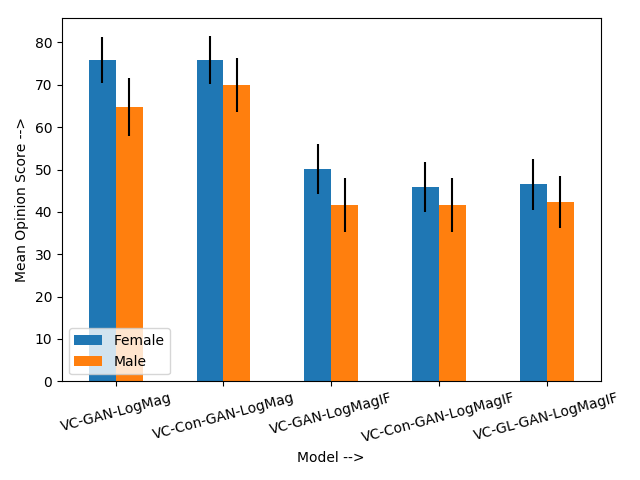
\includegraphics[width=6cm, height=6cm]{master_thesis_template/figs/quality(2).png}}}
    \qquad
    \subfloat[Domain]{{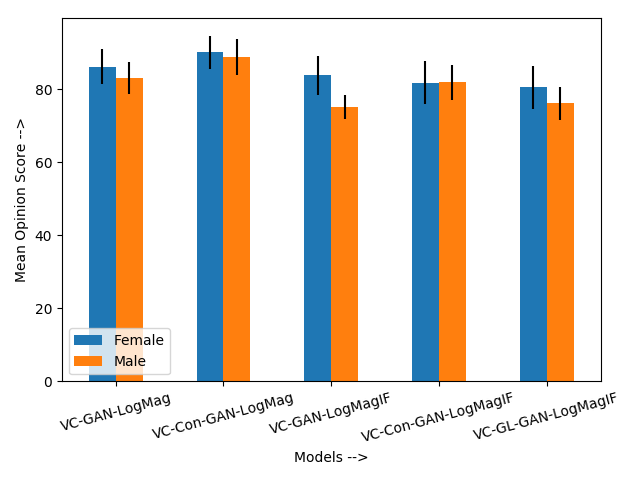
\includegraphics[width=6cm,height=6cm]{master_thesis_template/figs/domain(2).png}}}
    \caption[Mean opinion score]{Mean opinion score for the perceptual listening test}
    \label{fig:mos_quality_domain}
\end{figure}
\begin{table}[h]
    \centering
    \begin{tabular}{cccccc}
    \toprule
    \textbf{Method} & \textbf{Spectrogram} & \multicolumn{4}{c}{\textbf{MOS}} \\
    & & \multicolumn{2}{c}{Quality} & \multicolumn{2}{c}{Domain} \\
    & & Male&Female & Male&Female\\
    \midrule
    \textbf{VC-GAN} & LogMag & 64.66&76.28&82.62&87.18\\
                    &LogMagIF &45.46& 41.27&74.43&83.22 \\    
    \textbf{VC-Con-GAN}&LogMag & $\mathbf{70.13}$&$\mathbf{76.29}$& $\mathbf{88.44}$ & $\mathbf{89.50}$\\
    &LogMagIF &41.32&49.81&80.98&81.17\\
     \textbf{VC-GL-GAN} &LogMagIF&42.19&46.43&75.35&79.81 \\
    \bottomrule    
    \end{tabular}
    \caption[Mean Opinion Score]{Mean opinion scores}
    \label{tab:mos}
\end{table}

We further performed a Wilcoxon signed-rank test (\cite{wilcoxon1970critical}) to see the significance of the difference between VC-GAN and VC-Con-GAN. In particular, we evaluate whether the MOS of the two models for the same sample is similar. For the domain evaluation test, we get a p-value of $0.001865$ for female-to-male samples and p-value of $0.000181$ for male-to-female samples. This indicates the distribution of scores of the two models is significantly different. Likewise, we also performed the test for comparing the quality of samples of the two models. We get a p-value of $0.000078$ for female-to-male samples and a p-value of $0.476942$ for male-to-female speakers. This implies that the quality of the two models is comparable for male-to-female speakers but significantly different for female-to-male speakers. Together with the Wilcoxon test and the MOS, we conclude the VC-Con-GAN outperforms the VC-GAN for the domain translation task. Furthermore, it is also a clear winner for the quality of the generated male voice and is comparable to the VC-GAN for the quality of the generated female voice.

%Combinatorial problem to learn all possible combination of IF and magnitude. In addition, at any given point of time there are multiple frequency component present in the waveform. Thus to train a NN to generate full spectrogram representation requires a network to learn all possible right combination of phase and magnitude information. This is computationally intractable and makes it challenging to generate full spectrum representation.
